We have now seen that radiation pressure coupling between an optical mode and a mechanical mode can lead to laser cooling of the mechanical mode if the control beam $\bar{s}_{in}$ is tuned to the red sideband transition of the optomechanical system. If we now also introduce a weak probe beam, this leads to destructive interference for the excitation of an intra-cavity probe field with the mechanical induced sideband field when $\omega_p = -\Omega_m$, thus inducing a transparency window for the probe beam oscillating at $\omega_p = \omega_l + \Omega$ \cite{weis2010}. Optomechanical induced transparency (OMIT) can be used to slow light, but we use it as an extremely useful tool to experimentally obtain otherwise hard-to-get parameters such as light-enhanced optomechanical coupling $g = Gx_{zpf}\sqrt{\bar{n}_{cav}}$ and detuning $\Delta$. We also get more accessible parameters as the cavity linewidth $\kappa$ and mechanical frequency $\Omega_m$.

We will start out by solving this problem for a drive field $s_{in}(t) = (\bar{s}_{in} + \delta s_{in}(t))e^{i\omega_l t}$, the perturbation term $\delta s_{in}(t) = s_pe^{-i(\omega_p - \omega_l)t}$ will later be identified with the probe field in the linearized Heisenberg-Langevin equations. We assume that all the drives are weak classical coherent fields, resulting in all expectation values of operators will replaced with the classical term, e.g. $\langle\delta\hat{a}(t)\rangle \equiv \delta a(t)$. All quantum and thermal noise terms average to zero. We solve the coupled linearized equations of motion \eqref{eq:da}, \eqref{eq:dad} and \eqref{eq:dx} for the intra-cavity field $(\bar{a}^\dagger(\Omega)\delta\hat{a}(\Omega) + \bar{a}(\Omega)\delta\hat{a}^\dagger(\Omega))$. The analytic expression is to cumbersome to be shown here and obtain the solution using Mathematica. A theoretical prediction of the model is shown in figure \ref{fig:omit_theory_lol}.

\begin{figure}[H]
\centering
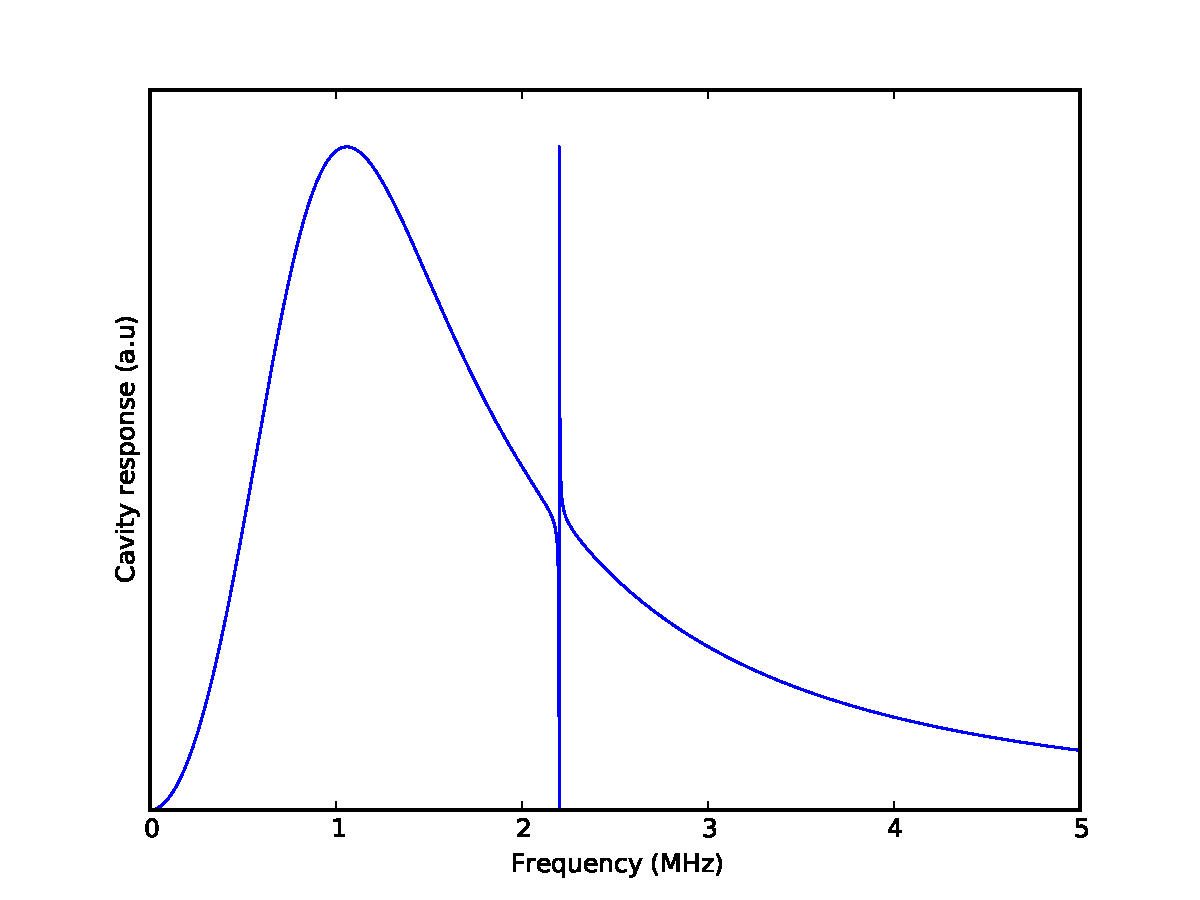
\includegraphics[scale=0.7]{omit_theory.pdf}
\caption{Theoretical prediction of the OMIT model, for $\kappa/2\pi = $ \SI{1.5}{\mega\hertz}, $\bar{\Delta} = -\kappa/2$, $\Omega_m/2\pi = 2.2$ \SI{}{\mega\hertz} and $g/2\pi = 100$ \SI{}{\kilo\hertz} .}
\label{fig:omit_theory_lol}
\end{figure}